\begin{figure}
	\centering
	\begin{subfigure}{0.8\textwidth}
		\centering
		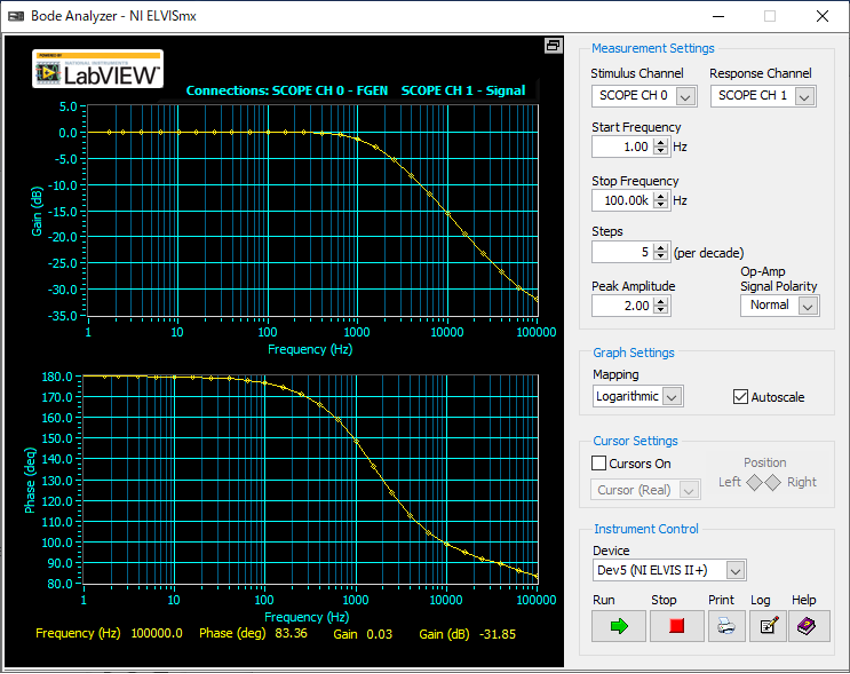
\includegraphics[width=0.8\linewidth]{src/figures/exp9/ope2-bode.png}
		\subcaption{オペアンプ2を用いたローパスフィルターのボード線図}\label{subfig:exp9-ope2-bode}
	\end{subfigure}
	\begin{subfigure}{0.8\textwidth}
		\centering
		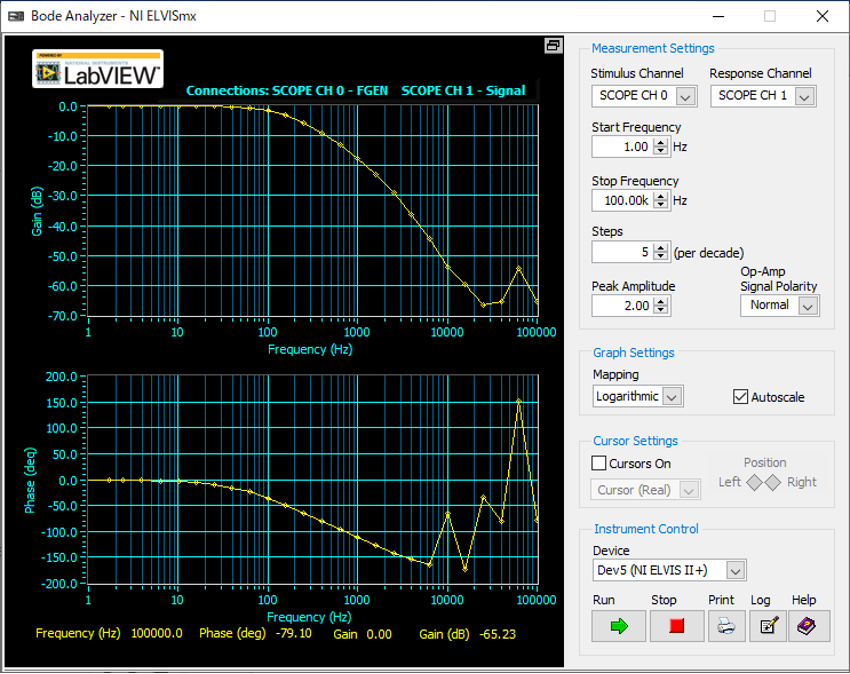
\includegraphics[width=0.8\linewidth]{src/figures/exp9/ope12-bode.png}
		\subcaption{オペアンプ1とオペアンプ2を継続接続したローパスフィルターのボード線図}\label{subfig:exp9-ope2-ope1-bode}
	\end{subfigure}
	\caption{実験9のボード線図}\label{fig:exp9-bode}
\end{figure}
